\section{Results}
\subsection{Min, Max, Average, and Median}
We had to determine whether the basic functionality of the system was working. We did this by continually testing the system during implementation. Here we present the proof that our system functions correctly and satisfies the first three requirements in the specification. We conducted ten runs of the four mathematical calculations specified in the assignment description. This experiment was conducted with a 16,382 node network. Finally, we limited the maximum number of gossip rounds to 200.

The average of all the runs fall within the target delta of less than or equal to 3\%. However, it is not enough to simple look at the average error. We also look at the standard deviation of error, the maximum and the minimum error. This is because of criteria for convergence is that every node's error is less than or equal to 3\%. Looking at the standard deviation of the error tells us how quickly we are converging. Looking and the min and max of the error gives us an indication when we have converged. Up to this point, we have talked about the error generically. Each of the mathematical calculations has its own error. 

\begin{figure}[ht!]
\centering
\setlength\fboxsep{0pt}
\setlength\fboxrule{0.5pt}
\fbox{
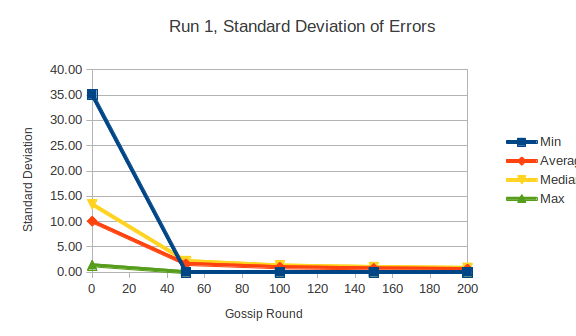
\includegraphics[width=90mm]{run1_stdev.png}
}
\caption{Plot of standard deviation of errors for Run 1.}
\label{fig:Run1_stdev}
\end{figure}


For the sake of brevity, the results of the first four runs are summarized in Appendix 5.1. One can see that as more and more rounds of gossip happen, the average error drops. The standard deviation of the error decreases as well. The maximum and minimum of errors approach zero as the number of rounds increases. Note minimum of errors of the average and median calculation during Run 1 at round 200. The average is -3.16 and the median is -4.1. In this particular case, those calculation have not converged to useful values based on our criteria. Allowing gossip to continue for those calculation would eventually yield correct answers, since one can see that the average, standard deviation (as shown in Figure \ref{fig:Run1_stdev}), min and max of the error during Run 1 are decreasing. 

The minimum and maximum calculation converge faster than the other two due to the distribution of their values. This phenomenon will be examined later.

The dependence of the convergence speed on the distribution of the data was alarming at first. However, with enough experimentation we can determine the bounds of the convergence speed. 

\subsection{Min and Max revisited}
After seeing the results of the first experiment, we thought it would be prudent to analyze the min and max calculation at a finer scale.The experimental setup was 16,382 nodes gossiping for 10 rounds. Each round was recorded and this experiment repeated ten times. Appendix 5.2 summarizes our findings and for the sake of brevity on the first run is shown. Figure \ref{fig:Run1_minmax} shows the characteristics of the min and max operations in relation to their errors at a finer scale. Comparing the rate of decrease of the standard deviation between the various calculations, the minimum's standard deviation clearly decreases faster than any other (Figure \ref{fig:Run1_stdev_minmax}). Looking at the max and min of all errors tells us something interesting. Although the minimum is quickly converging, there remains at least one node whose answer is way off (Figure \ref{fig:Run1_max_errors} and \ref{fig:Run1_min_errors}).


\begin{figure}[ht!]
\centering
\setlength\fboxsep{0pt}
\setlength\fboxrule{0.5pt}
\fbox{
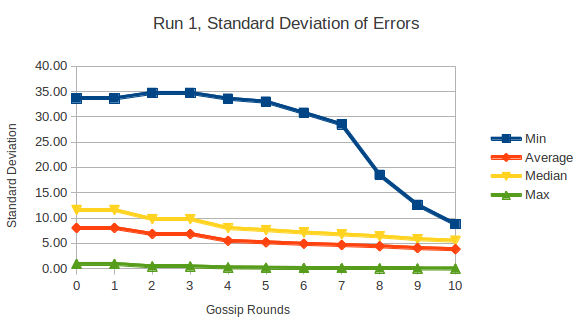
\includegraphics[width=90mm]{run1_stdev_minmax.png}
}
\caption{Plot of standard deviation of errors for Run 1, min/max revisited.}
\label{fig:Run1_stdev_minmax}
\end{figure}

\begin{figure}[ht!]
\centering
\setlength\fboxsep{0pt}
\setlength\fboxrule{0.5pt}
\fbox{
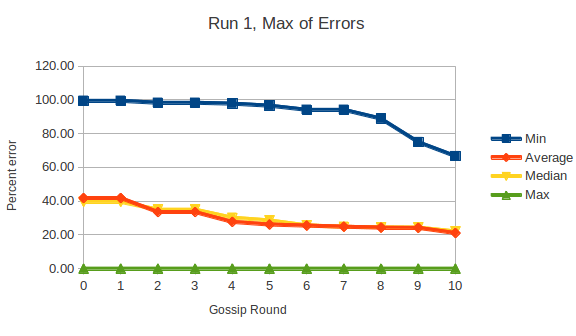
\includegraphics[width=90mm]{run1_max_error.png}
}
\caption{Plot of max of errors for Run 1, min/max revisited.}
\label{fig:Run1_max_errors}
\end{figure}

\begin{figure}[ht!]
\centering
\setlength\fboxsep{0pt}
\setlength\fboxrule{0.5pt}
\fbox{
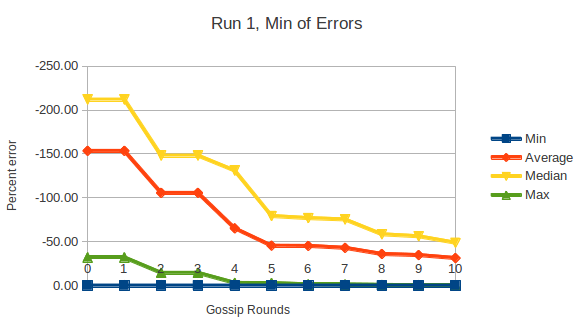
\includegraphics[width=90mm]{run1_min_error.png}
}
\caption{Plot of min of errors for Run 1, min/max revisited.}
\label{fig:Run1_min_errors}
\end{figure}

\subsection{Scalability}
To test how well our system scales, we conducted experiments with different number of nodes. The results of the experiments are summarized in Figure \ref{fig:scalability}. As the number of nodes in the system increases, the time to converge per node decreases. 

\begin{figure}[ht!]
\centering
\setlength\fboxsep{0pt}
\setlength\fboxrule{0.5pt}
\fbox{
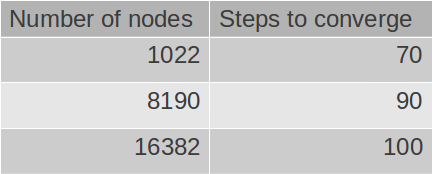
\includegraphics[width=90mm]{scalability.png}
}
\caption{}
\label{fig:scalability}
\end{figure}

\subsection{Fragments}
We also show proof that 4th and 5th requirements are fulfilled by running examples of updating and retrieving fragment data. A network of 16,382 nodes was created and fragments were initialized at each node with pseudo-random data. An arbitrary fragment number was chosen to be updated. The system was passed a new set of data for the fragment to be stored at the destination nodes containing the fragment. The update started at node 1 and the number of gossip rounds needed to store the fragment was recorded. Out of 100 trials it took an average of 896 rounds of gossip to store the fragment.

Retrieving fragment data was tested on the same network. Data from an arbitrary fragment was requested from node 1. The number of gossip rounds it took to retrieve the fragment was recorded. Out of 100 trials it took an average of 529 rounds of gossip to retrieve the fragment.

\subsection{Spawning Nodes on Remote Machines}
Erlang allows for easy spawning of processes on a remote machine. We were able to take advantage of this to spawn nodes on another Erlang interpreter running on a seperate VM with only slight modification of the code. Both VMs need to have the code compiled and the Erlang interpreter running.

The functions for spawning nodes were modified to spawn every other node on the remote system. The network generation was done in the same way as when using a single VM, so the nodes have the same degree as the single system implementation (3 for most nodes). Because of this, all functions required approximately the same number of gossip rounds to converge. However, due to additional latency introduced by the network communication, operations took roughly twice as long to complete.

